\documentclass[conference]{IEEEtran}
\IEEEoverridecommandlockouts
% The preceding line is only needed to identify funding in the first footnote. If that is unneeded, please comment it out.
\usepackage{cite}
\usepackage{amsmath,amssymb,amsfonts}
\usepackage{algorithmic}
\usepackage{graphicx}
\usepackage{listings}
\usepackage{textcomp}
\usepackage[dvipsnames]{xcolor}
\def\BibTeX{{\rm B\kern-.05em{\sc i\kern-.025em b}\kern-.08em
    T\kern-.1667em\lower.7ex\hbox{E}\kern-.125emX}}
\usepackage{caption}
\usepackage{subcaption}
% \usepackage{slashbox}
\usepackage{diagbox}
\begin{document}

\title{Decomposing Sums of Sines by using Artificial Evolution\\
% {\footnotesize \textsuperscript{*}Note: Sub-titles are not captured in Xplore and should not be used}
}

\author{\IEEEauthorblockN{Ali Khudiyev}
\IEEEauthorblockA{\textit{Data Science and Artificial Intelligence} \\
\textit{French-Azerbaijani University}\\
Baku, Azerbaijan \\
ali.khudiyev@ufaz.az}
}

\maketitle

\begin{abstract}
	Strategies of artificial evolution have been widely used for various optmization problems which include some hard engineering problems. The concern of this paper is to decompose a given signal into 
	summation of arbitrary number of sine waves by using one of such stragies. While Fourier transform is able to decompose such given signals into infinite number of sine waves, we want to control the 
	number of sines that are used to reconstruct the originial signal with the minumum loss. For this purpose, I introduce the proposed evolutionary algorithm in terms of some essential implementation details. 
	Experimental setup and results are shared and discussed thoroughly before getting to the final conclusions. During the development process, I try to find experimentally supported answers to several 
	interesting questions such as the effect of amplitude, freqeuncy and phase shift on the quality of approximation, respective distances between original sine waves and the approximating signal and so on.
\end{abstract}

\begin{IEEEkeywords}
	Artificial Evolution, Metaheuristics, Optimization, Signal Processing 
\end{IEEEkeywords}

\section{Introduction}
\textit{Artificial Evolution} is defined as any procedure which uses stragies of Darwinian evolution. In computer science, these strategies are widely used for various optimization problems where the problem 
consists of concepts that are interconnected in some high dimensional space which are very hard to solve manually by developing a non-stochastic algorithms. The deveoped algorithms are also known as 
Genetic Algorithms (GAs) or Evolution Programming which is essentially for exploring and exploiting any search space in order to find the globally minimum cost value determined by the given objective 
function. Implementation of such algorithms uses 3 main processes of the Darwininan evolution which are \textit{mutation}, \textit{crossover} and \textit{selection}.

Genetic algorithms \cite{ga} is one of the many metaheuristics which is used to obtain high quality solutions for optimization problems by relying on the previously mentioned 3 operations. 
One of the main reasons to use such metaheuristics is because they do not require any assumptions or constraints about the problem that they are applied to solve. In other words, these algorithms 
are generic and can be applied to any problem as long as encoding of the problem is suitable. However, there are several challanges that we may encounter when using metaheuristics such as using 
the optimal set of hyperparameters for a specified problem or a way to not get stuck at local minimums of the objective function to be minimized. The tendency to converge to a local optima can 
be potentially avoided by increasing diversity(mutation rate) but there is no general way solving this problem due to \textit{No Free Lunch} theorem. Another potential problems are repeated 
cost or objective function evaluations for complex problems as some real-world objectives can take from several hours to several days to be computed, non-effective approach for solving problems 
with binary fitness values(e.g., decision problems) and poor ability of not scaling well with the complexity due to the exponential increase in search space by relatively large number of elements 
exposed to mutation.

\subsection{Problem Statement}
The concern of this paper is to use one proposed GA to solve a problem which is about decomposing a given signal to arbitrary number sine waves with the least loss possible. First, the original 
signal is constructed by some pre-defined composition of one or more $\sin$ functions and then data is collected by plugging in different $x$ input values. The collected data is given to the proposed 
algorithm to compute the loss of approximated signal. The figure \ref{fig:example} illustrates a simple signal made up from the composition of two sine signals with different amplitude, frequency 
and phase shift.

\begin{figure}[h]
	\centering
	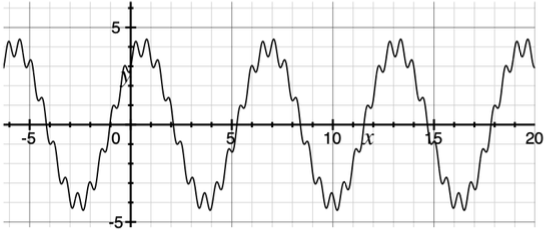
\includegraphics[width=0.75\linewidth]{img/example.png}
	\caption{$f(x) = \frac{1}{2}\sin(11x-1) + 4\sin(x+1)$}
	\label{fig:example}
\end{figure}

There are several questions to which I try to provide answers in this paper. They are the following:

\begin{enumerate}
	\item Which amplitude, frequency and phase shift values are to be found to minimize the loss function?
	\item What is behaviour of the algorithm when we try to approximate a signal with several sine functions with only a single sine function?
	\item What is bahaviour of the algorithm when we try to approximate a signal with $n$ sine functions with $s$ sine functions?
\end{enumerate}

These questions help to get a better idea about the overall behaviour of the proposed genetic algorithm by questioning the nature of found approximations. I also want to mention that the provided answers 
are strongly experiment based as the program has been run on several example signals(e.g., figure \ref{fig:example}) with different hyperparameters and cost evaluation strategies.

\subsubsection{Mathematical formulation}
To approximate the given function $f(x)$, we want to minimize the cost function shown below:

\begin{equation}
	C = \frac{1}{n} \sum_{i=1}^{n} |y_i-\hat{y}_i|
	\label{eq:cost}
\end{equation}

where $n$ is the number of samples. However, absolute value function is continous but not differentiable at any point which makes it hard to find gradients on such cost function in order to find 
the minimum of the function. Due to this reason, we can transform $C$ to $L$ such that minimization of $L$ guarantees the minimization of $C$ while $L$ being differentiable and therefore, continuous. 
Such loss function could be written as shown below:

\begin{equation}
	L = \sum_{i}^{n} (y_i-\hat{y}_i)^2 = \sum_{x \in X}^{} (f(x)-a\sin(bx+c))^2
	\label{eq:loss}
\end{equation}

where $X$ is the subdomain with finite cardinality of the function. To find local/global minimums of $L$, we need to differentiate it with respect to 3 independent variables $a$ for amplitude, $b$ for 
frequency and $c$ for phase shift.

\begin{align*}
	\frac{\partial L}{\partial a} &= \sum_{x}^{} -2(f(x)-a\sin(bx+c))\sin(bx+c) \\
	\frac{\partial L}{\partial b} &= \sum_{x}^{} -2(f(x)-a\sin(bx+c))a\cos(bx+c)x \\
	\frac{\partial L}{\partial c} &= \sum_{x}^{} -2(f(x)-a\sin(bx+c))a\cos(bx+c)
	\label{eq:dervs}
\end{align*}

Solving the set of equalities where $\frac{\partial{L}}{\partial{a}} = \frac{\partial{L}}{\partial{b}} = \frac{\partial{L}}{\partial{c}} = 0$ would give us amplitude, frequency and phase shift 
values which are the optimal solutions for for the decomposition problem. By using GA, we are actually solving this set of equations iteratively in a numerical way.

\section{State of The Art}
Signal processing is one of important fields of study due to its various applications such as texture analysis, fractal analysis, image compression and so on. There are several methods known as 
\textit{Emprical Mode Decomposition} (\textit{EMD}) \cite{emd}, \textit{Variational Mode Decomposition} (\textit{VMD}) \cite{vmd}, \textit{Hilber Vibration Decomposition} (\textit{HVD}) \cite{hvd}, 
etc. which are used to process and decompose signals. The EMD method is a fundamental part of \textit{Hilbert-Huang Transform} (\textit{HHT}) and it decomposes a given signal into finite number of 
components which are also known as \textit{intrinsic mode functions} (\textit{IMF}). On the other hand, HVD separates a signal from the initial vibration which contains the varying highest amplitude 
as the first component resulting with the residual signal that contains other lower amplitude components. This strategy also has much higher frequency resolution than the EMD method. VMD has been 
proposed by Konstantin Dragomiretskiy and Dominique Zosso as an adaptive, fully intrinsic, variational method which represents decomposition of a signal into its principal modes by minimization.

Fourier Transform (FT) \cite{ft,ft2} is a widely used mathematical transform to decompose functions into functions with the specified spatial or temporal frequencies. Such strategy would take any signal 
and find out the $\sin$ and $\cos$ functions with some coefficients whose composition makes up the originial signal.

\begin{align*}
	\hat{f}(\xi) = \int_{-\infty}^{\infty} f(x) e^{-2\pi ix\xi} dx
	% \label{eq:ft}
\end{align*}

where $\xi$ is the frequency given in Hz and $x$ represents time in seconds. Although there lies powerful and beautiful theory behind FTs, they are to find infinite number of signals with different 
frequencies. This means that there is no direct way of asking FTs to decompose a signal to a given number of sines. In addition to this, it is also impossible to provide the FT strategy with a 
knowledge base which would potentially boost the run-time performance of the signal decomposition process.

Genetic Algorithm (GA) \cite{ga1,ga2,ga3} has been used for different optimization problems and it has shown promising results. Due to this, there is a huge potential to develop such evolutionary 
approach for signal processing as well. Decomposition of a signal is also an optimization problem for decreases the loss by adjusting the independent variables known as amplitude, frequency and phase. 
Some applications of GAs include vehicle routing problem (VRP) (e.g., traveling salesman problem), scheduling tasks, feature selection for machine learning (ML), creativity of artificial intellgence (AI), 
controlling systems for robotics, image processing and so on.

\section{Implementation Details}
EASEA (EAsy Specification of Evolutionary Algorithms) \cite{easea} is an Artificial Evolution platform which enables scientists, who are not either experienced or interested in programming, to develop 
solutions to the problems of their domains by using significantly few lines of codes. The platform helps people to focus on their problems more than the implementation details as it provides massive 
parallelism by using GPGPUs or even several locally connected computers. EASEA has been developed by BFO team at Strasbourg University and according to the developers, it can enable up to x1000 performance 
boost although it is common to get speedups in the interval of x100-x1000.

The proposed algorithm for this project has been developed on EASEA by using one of its templates. There are several headers that the template file contains most of which are self-explanatory. For example, 
\textbf{User declarations} header is used to define preprocessor macros or declare variables, statements or functions defined in \textbf{Before everything else} and \textbf{After everything else} headers 
are to be executed at the entry and end of the program respectively, \textbf{User classes} header is used to define custom data structure to hold the candidate solutions. Once the user defines the custom 
data structure \textbf{S}, \textbf{S::initializer}, \textbf{S::crossover}, \textbf{S::mutator} and \textbf{S::evaluator} headers are defined to specify the process of initialization, crossover, mutation and 
evaluation respectively. Finally, \textbf{Default run parameters} header is filled with the default number of generations, time limit, population size, offspring size, mutation and crossover probability, 
and so on.

\subsection{Mutation}
When a selected individual goes through the mutation process, amplitude, frequency and phase shift values of the individual are updated by adding randomly generated $\Delta \text{amp}$, 
$\Delta \text{freq}$ and $\Delta \text{ph}$ in the intervals of $[-10,10)$, $[-1,1)$ and $[-0.628,0.628)$ respectively. Updated values go through the process of boundary checking which sets 
them to the nearest boundary value if the boundary conditions are violated. Adding the generated values to the old values makes individuals explore their surrounding rather than a completely 
random points. With the current settings, a gene(amplitude, frequency or phase shift) can potentially explore 20\% of its surrounding by mutating.

\subsection{Crossover}
After generating random \textbf{nLocus} value, some genes of the selected children are replaced by the genes of their parents. While performing the crossover, replaced genes can only be triplets of (amplitude, 
frequency, phase shift) since these are the genes which are grouped together and used for single sine function. Such implementation helps the algorithm to generally converge better without creating a lot of 
children with poor fitness values.

\subsection{Selection}
Selection process of individuals is based on their fitness values which is computed in the \textbf{evaluation} header. To evaluate individual's fitness value, the loss is computed as the mean absolute difference 
between points of the target and approximating signals which gives us information about the expected loss of candidate signal at any point of time. Fitness values are computed by taking only 70\% of original 
points of the given signal and the rest 30\% is saved for validation/testing purpose. Since the goal is to obtain better approximations, \textbf{evaluator goal} is set to \textit{minimise} as the default run 
parameter.

\section{Experiments}
\subsection{Experimental Setup}
Experiments have been carried on an Ubuntu 20.04 machine with 3.2GHz CPU and 16GB RAM. The algorithm has been run only sequentially without using any GPU parallelism. Apart from the example signal 
$f_2(x) = \frac{1}{2}\sin(11x-1) + 4\sin(x+1)$, random signals with 3, 5 and 8 sines have been generated to collect 1000 data points 70\% of which is used to evolve generations and the rest 30\% for 
testing the best candidate obtained in the last generation. For the robustness of tests, statistical data is provided after 30 runs after which I provide answers to the main questions of the paper.
The number of generations is set to 100 without any program run-time limit constraint.

\subsection{Results}
Equation \ref{eq:f3} is the selected target signal with 3 sines and the figure \ref{fig:sin3_1} illustrates the evolution history of a set of single sines and finally the plot of original/target signal and 
obtained sine. The mean fitness(loss) values start from 53-55 and drops to 20-22 while the best fitness drops to 15-16 by less than 100 number of generations. Plot \ref{fig:plot_sin3_1} shows that
the approximating sine function tries to match the frequency and phase shift of the biggest sine in original signal.

\begin{equation}
	f_3 = f_2 - 12\sin(-3.5x-4)
	\label{eq:f3}
\end{equation}

\begin{equation}
	f_3^1 = 12.193\sin(3.499x+4.076)
	\label{eq:f3_pred}
\end{equation}

\begin{figure}[h]
\centering
\begin{subfigure}{.8\linewidth}
  \centering
  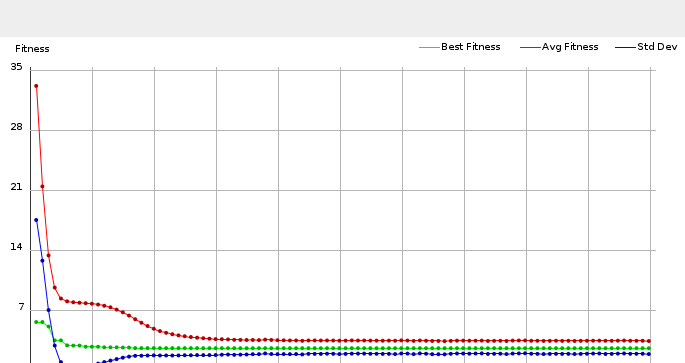
\includegraphics[width=.9\linewidth]{img/sin3_1_new.png}
  \caption{Evolution history}
  \label{fig:hist_sin3_1}
\end{subfigure}

\begin{subfigure}{.8\linewidth}
  \centering
  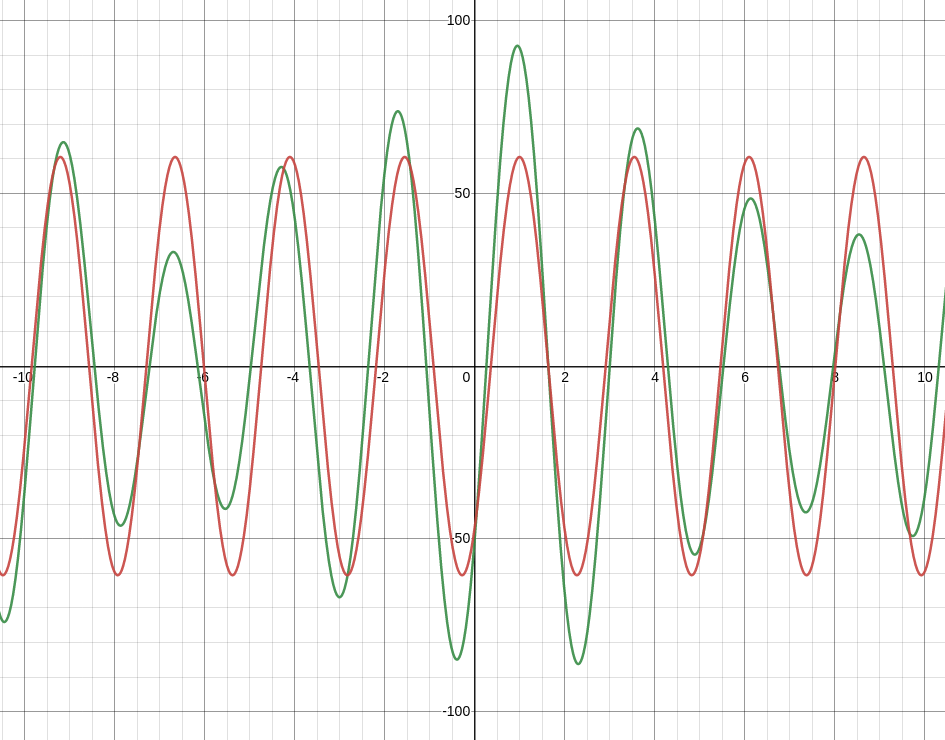
\includegraphics[width=.9\linewidth]{img/plot_sin3_1.png}
  \caption{Plot of \textcolor{ForestGreen}{$f_3$} and \textcolor{red}{apprximating sine}}
  \label{fig:plot_sin3_1}
\end{subfigure}
\caption{Approximating 3 sines by using 1 sine}
\label{fig:sin3_1}
\end{figure}

Equation \ref{eq:f5} shows the formula of a signal with 5 sine waves and the figure \ref{fig:sin5_1} illustrates the evolution history of a set of single sines and the final plots. Unlike apprxomating 
sum of 3 sines with a single sine, average fitness, the best fitness and standard deviation is highger through the evolutions of sine waves since it is hard to approximate such a ``noisy signal'' with 
only one sine function. However, the results are similar in terms of the amplitude, frequency and phase shift of the obtained sine function which are closer to the biggest sine used in the target signal.

\begin{equation}
	\begin{split}
		f_5 =& f_2 + 78\sin(-3.5x-4) \\
		&- 53\sin(15x-3.3) + 48.3\sin(5.8x+2) \\
	\end{split}
	\label{eq:f5}
\end{equation}

\begin{equation}
	f_5^1 = 83.67\sin(3.49x+4.07)
	\label{eq:f5_1}
\end{equation}

\begin{figure}[h]
\begin{subfigure}{.8\linewidth}
  \centering
  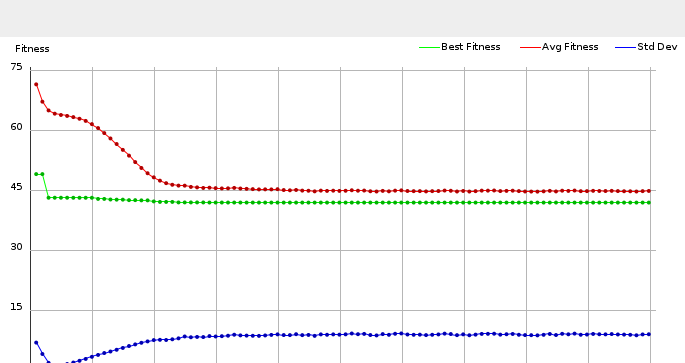
\includegraphics[width=.9\linewidth]{img/sin5_1_new.png}
  \caption{Evolution history}
  \label{fig:hist_sin5_1}
\end{subfigure}

\begin{subfigure}{.8\linewidth}
  \centering
  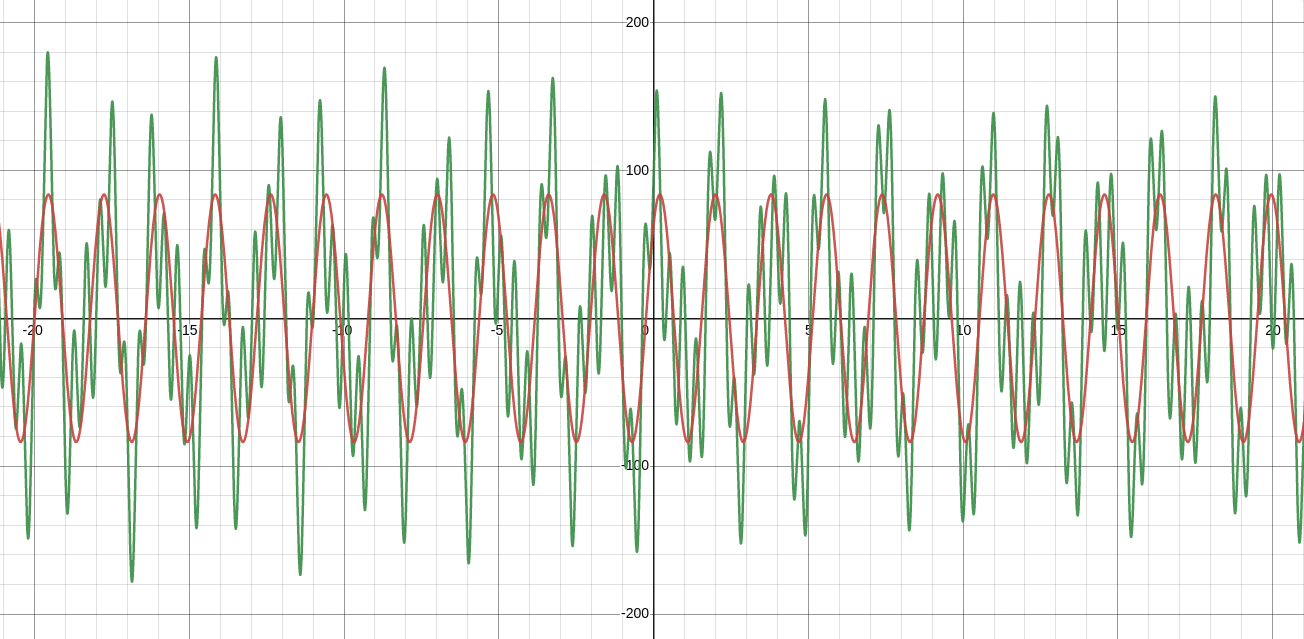
\includegraphics[width=.9\linewidth]{img/plot_sin5_1_new.png}
  \caption{Plot of \textcolor{ForestGreen}{$f_5$} and \textcolor{red}{approximating sine}}
  \label{fig:plot_sin5_1}
\end{subfigure}
\caption{Approximating 5 sines by using 1 sine}
\label{fig:sin5_1}
\end{figure}

Equation \ref{eq:f8} is another example arbitrary target signal and figure \ref{fig:sin8_1} illustrates its evolution history and the final plots. The same results observed for $f_5$ and $f_3$ are observed 
for this function as well and it has become more obvious that any sine wave with the biggest amplitude contributes to the signal more than the others do in general. From the plot \ref{fig:plot_sin8_1} we 
can also observe that the convergence emerges way before reaching 100 generations. The convergence point is almost the same when we try to approximate 3, 5 and 8 sines by using a single sine.

\begin{equation}
	\begin{split}
		f_8 =& f_2 - 78\sin(-3.5x-4) - 53\sin(5x-3.3) \\
			&+ 48.3\sin(5.8x+2) + 10\sin(8x+6.1) \\
			&+ 92\sin(-x+3.6) - 3\sin(x+4.2)
	\end{split}
	\label{eq:f8}
\end{equation}

\begin{equation}
	f_8^1 = 96.143\sin(x+5.847)
	\label{eq:f8_1}
\end{equation}

\begin{figure}[h]
\centering
\begin{subfigure}{.8\linewidth}
  \centering
  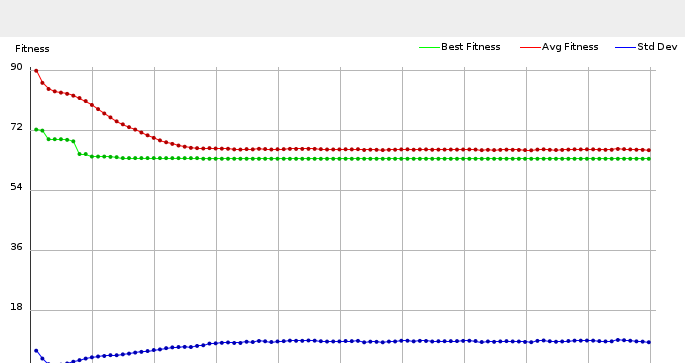
\includegraphics[width=.9\linewidth]{img/sin8_1_new.png}
  \caption{Evolution history}
  \label{fig:hist_sin8_1}
\end{subfigure}

\begin{subfigure}{.8\linewidth}
  \centering
  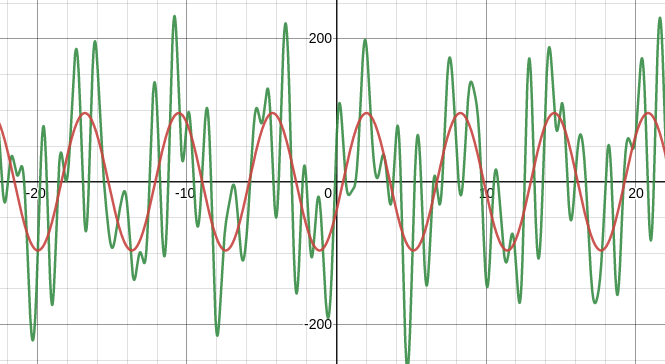
\includegraphics[width=.9\linewidth]{img/plot_sin8_1_new.png}
  \caption{Plot of \textcolor{ForestGreen}{$f_8$} and \textcolor{red}{approximating sine}}
  \label{fig:plot_sin8_1}
\end{subfigure}
\caption{Approximating 8 sines by using 1 sine}
\label{fig:sin8_1}
\end{figure}

Figure \ref{fig:sin3_2} illustrates what happens when we try to approximate the signal $f_3$ by using 2 sines instead of one. Unlike the previous cases, where we are allowed to use only 1 sine for approximation, 
the convergence is a bit delayed although it happens by less than 100 generations. This is normal due to the bigger search space with 6 variables as opposed to only 3(i.e., amplitude, frequency, phase shift).

\begin{equation}
	f_3^2 = 11.99\sin(3.5x+3.98) - 4.06\sin(x+4.02)
	\label{eq:f3_2}
\end{equation}

\begin{figure}[h]
\centering
\begin{subfigure}{.8\linewidth}
  \centering
  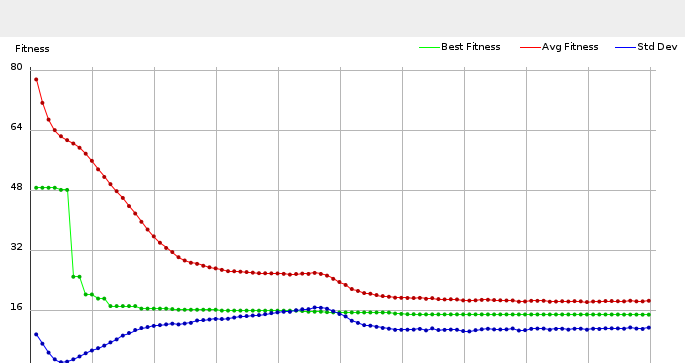
\includegraphics[width=.9\linewidth]{img/sin3_2.png}
  \caption{Evolution history}
  \label{fig:hist_sin3_2}

\end{subfigure}
\begin{subfigure}{.8\linewidth}
  \centering
  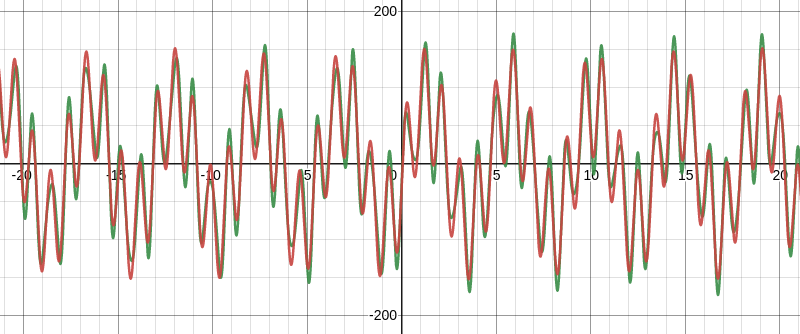
\includegraphics[width=.9\linewidth]{img/plot_sin3_2.png}
  \caption{Plot of \textcolor{ForestGreen}{$f_3$} and \textcolor{red}{approximating sines}}
  \label{fig:plot_sin3_2}
\end{subfigure}
\caption{Approximating 3 sines by using 2 sines}
\label{fig:sin3_2}
\end{figure}

Figure \ref{fig:sin5_3} illustrates what happens when we try to approximate the signal $f_5$ by using 3 sines.

\begin{equation}
	\begin{split}
		f_5^3 =& 14.63\sin(0.06x+6.84) + 74.1\sin(3.49x+0.91) \\
			&+ 43.8\sin(5.79x+2.14)
	\end{split}
	\label{eq:f5_3}
\end{equation}

\begin{figure}[h]
\begin{subfigure}{.8\linewidth}
  \centering
  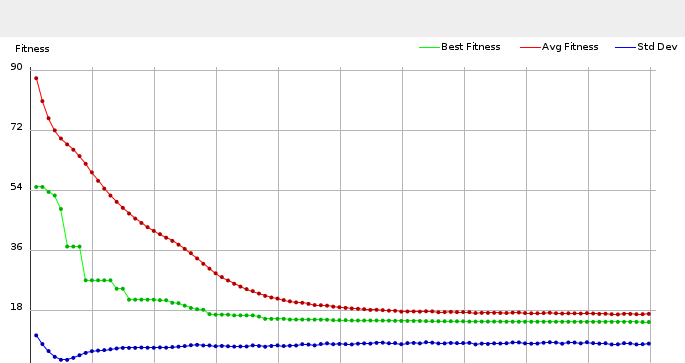
\includegraphics[width=.9\linewidth]{img/sin5_3.png}
  \caption{Evolution history}
  \label{fig:hist_sin5_3}
\end{subfigure}

\begin{subfigure}{.8\linewidth}
  \centering
  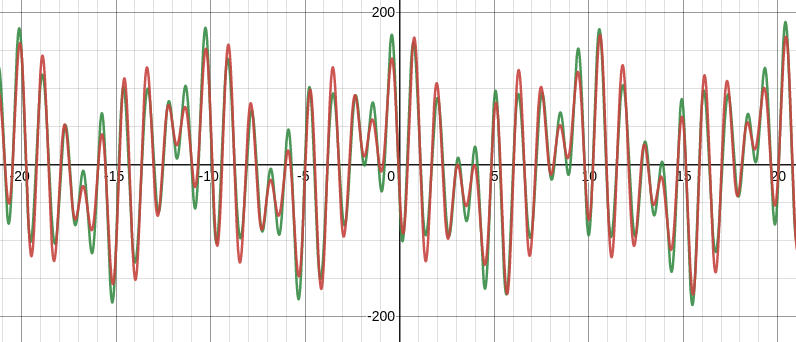
\includegraphics[width=.9\linewidth]{img/plot_sin5_3.png}
  \caption{Plot of \textcolor{ForestGreen}{$f_5$} and \textcolor{red}{approximating sines}}
  \label{fig:plot_sin5_3}
\end{subfigure}
\caption{Approximating 5 sines by using 3 sines}
\label{fig:sin5_3}
\end{figure}

Figure \ref{fig:sin8_5} illustrates what happens when we try to approximate the signal $f_8$ by using 5 sines.

\begin{equation}
	\begin{split}
		f_8^5 =& 35.94\sin(3.49x+1.26) + 44.25\sin(3.5x+0.52) \\
		&+ 47.66\sin(5.8x+1.91) + 52.81\sin(4.99x-0.01) \\
		&+ 92.27\sin(0.99x+5.96)
	\end{split}
	\label{eq:f8_5}
\end{equation}

\begin{figure}[h]
\centering
\begin{subfigure}{.8\linewidth}
  \centering
  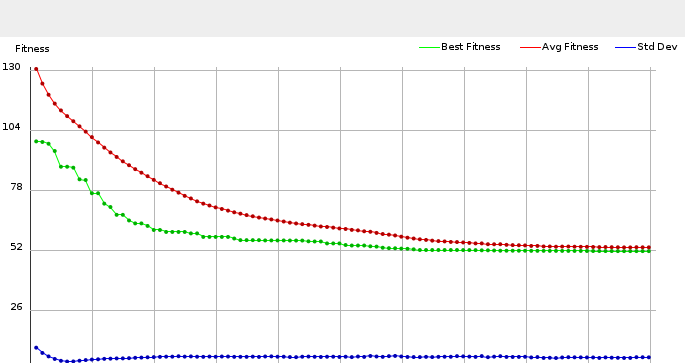
\includegraphics[width=.9\linewidth]{img/sin8_5.png}
  \caption{Evolution history}
  \label{fig:hist_sin8_5}
\end{subfigure}

\begin{subfigure}{.8\linewidth}
  \centering
  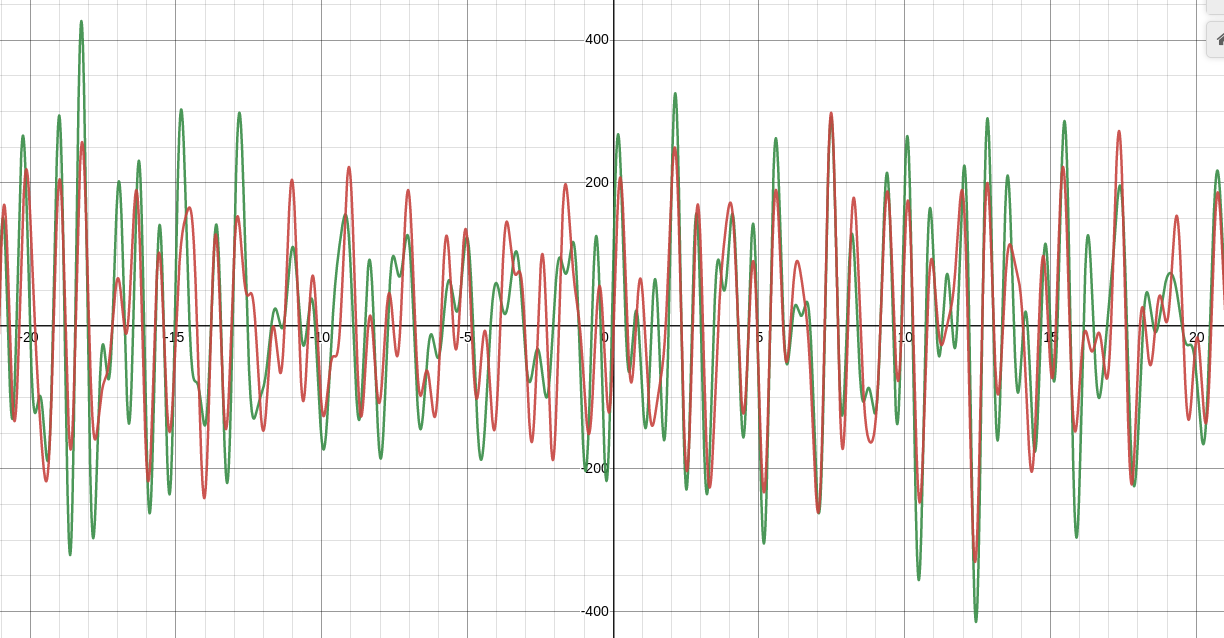
\includegraphics[width=.9\linewidth]{img/plot_sin8_5.png}
  \caption{Plot of \textcolor{ForestGreen}{$f_8$} and \textcolor{red}{approximating sines}}
  \label{fig:plot_sin8_5}
\end{subfigure}
\caption{Approximating 8 sines by using 5 sines}
\label{fig:sin8_5}
\end{figure}

Figure \ref{fig:sin2_3} illustrates what happens when we try to approximate the signal $f_2$ by using 3 sines which is clearly more than the number of sine waves in the original signal.

\begin{equation}
	\begin{split}
		f_2^3 =& 0.9\sin(1.01x+0.51) + 3.09\sin(0.99x+1.15) \\
		&- 0.14\sin(7.98x+2.95)
	\end{split}
	\label{eq:f2_3}
\end{equation}

\begin{figure}[h]
\centering
\begin{subfigure}{.8\linewidth}
  \centering
  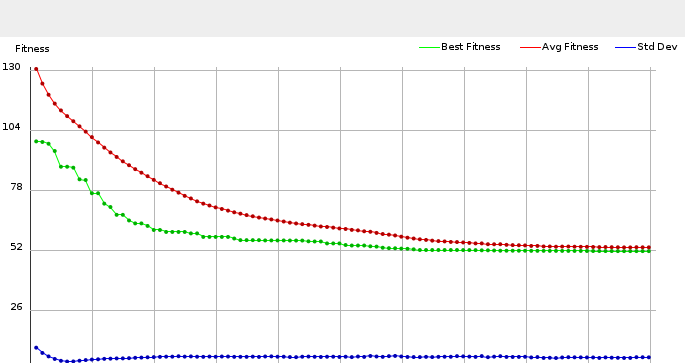
\includegraphics[width=.9\linewidth]{img/sin8_5.png}
  \caption{Evolution history}
  \label{fig:hist_sin2_3}
\end{subfigure}

\begin{subfigure}{.8\linewidth}
  \centering
  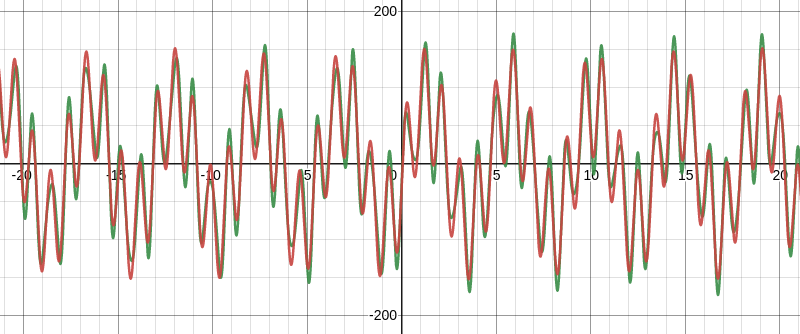
\includegraphics[width=.9\linewidth]{img/plot_sin3_2.png}
  \caption{Plot of \textcolor{ForestGreen}{$f_2$} and \textcolor{red}{approximating sines}}
  \label{fig:plot_sin2_3}
\end{subfigure}
\caption{Approximating 2 sines by using 3 sines}
\label{fig:sin2_3}
\end{figure}

Figure \ref{fig:sin3_5} illustrates what happens when we try to approximate the signal $f_3$ by using 5 sines.

\begin{equation}
	\begin{split}
		f_3^5 =& 0.58\sin(0.98x+2.31) + 3.47\sin(x+7.13) \\
			&+ 13.16\sin(3.5x+4.08) - 1.44\sin(3.49x+4.93) \\
			&+ 0.02\sin(-1.3x+3.66)
	\end{split}
	\label{eq:f3_5}
\end{equation}

\begin{figure}[h]
\centering
\begin{subfigure}{.8\linewidth}
  \centering
  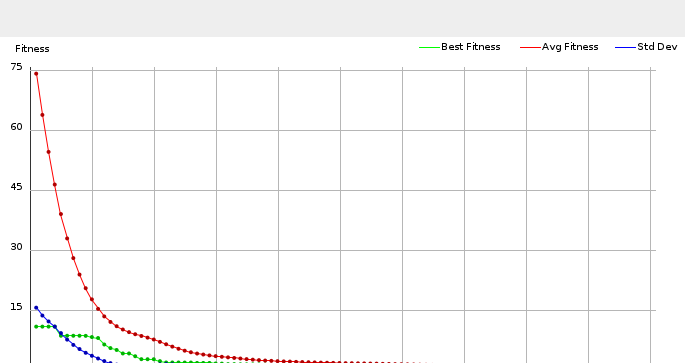
\includegraphics[width=.9\linewidth]{img/sin3_5_new.png}
  \caption{Evolution history}
  \label{fig:hist_sin3_5}
\end{subfigure}

\begin{subfigure}{.8\linewidth}
  \centering
  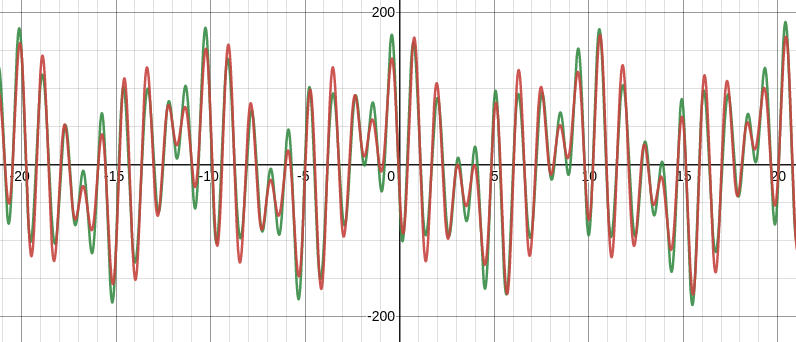
\includegraphics[width=.9\linewidth]{img/plot_sin5_3.png}
  \caption{Plot of \textcolor{ForestGreen}{$f_3$} and \textcolor{red}{approximating sines}}
  \label{fig:plot_sin3_5}
\end{subfigure}
\caption{Approximating 3 sines by using 5 sines}
\label{fig:sin3_5}
\end{figure}

Figure \ref{fig:sin5_8} illustrates what happens when we try to approximate the signal $f_5$ by using 8 sines.

\begin{equation}
	\begin{split}
		f_5^8 =& 33.76\sin(3.48x+1.97) + 8.83\sin(1.25x+5.34) \\
			&+ 9.41\sin(6.58x+0.68) + 10.87\sin(5.07x+3.81) \\
			&+ 9.28\sin(1.96x+5.24) + 39.2\sin(5.8x+1.78) \\
			&+ 11.02\sin(0.56x+0.52) + 57\sin(3.5x+0.35)
	\end{split}
	\label{eq:f5_8}
\end{equation}

\begin{figure}[h]
\centering
\begin{subfigure}{.8\linewidth}
  \centering
  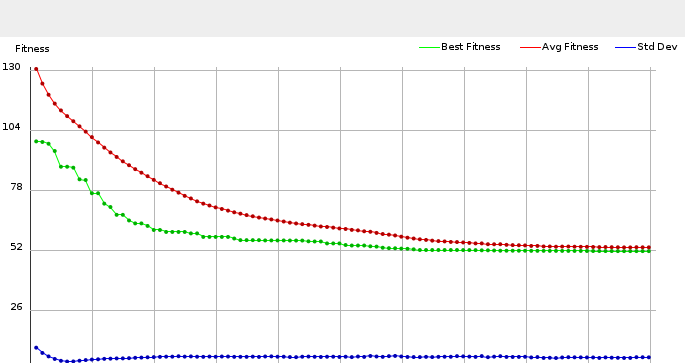
\includegraphics[width=.9\linewidth]{img/sin8_5.png}
  \caption{Evolution history}
  \label{fig:hist_sin5_8}
\end{subfigure}

\begin{subfigure}{.8\linewidth}
  \centering
  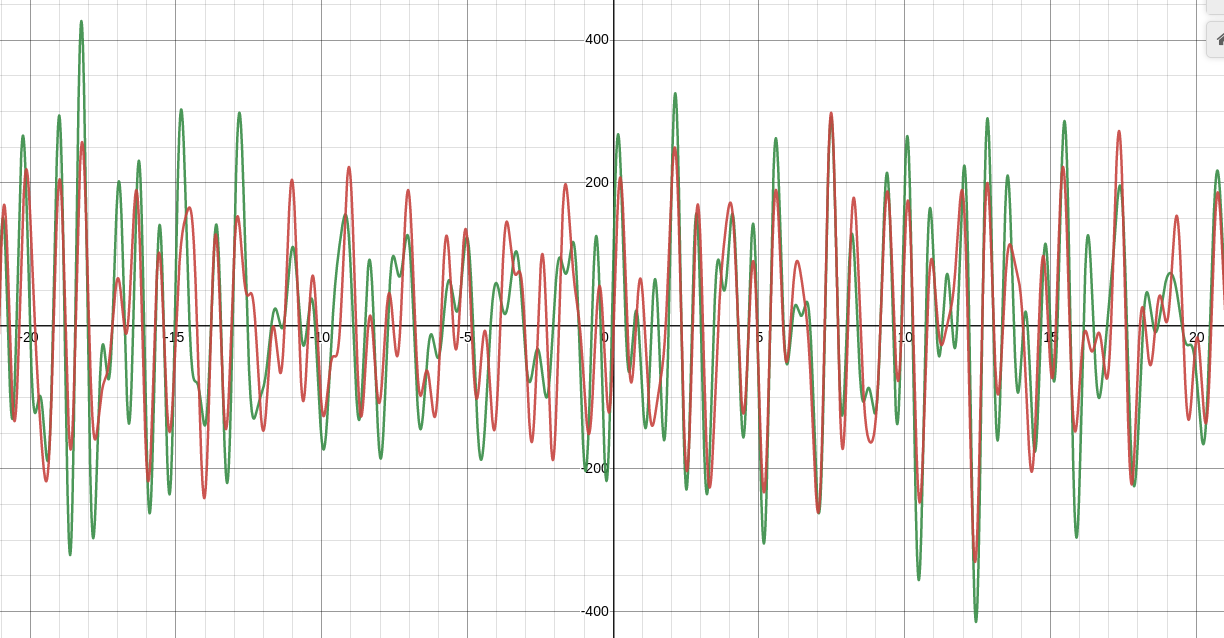
\includegraphics[width=.9\linewidth]{img/plot_sin8_5.png}
  \caption{Plot of \textcolor{ForestGreen}{$f_5$} and \textcolor{red}{approximating sines}}
  \label{fig:plot_sin5_8}
\end{subfigure}
\caption{Approximating 5 sines by using 8 sines}
\label{fig:sin5_8}
\end{figure}

Finally, 4 functions with 2, 3, 5, 8 sines have been set as targets and each of them is approximated with 1, 2, 3, 5 sines repeatedly for 15 runs. In total, the program has been executed for 240 times. 
Table \ref{tab:stats} shows the obtained results and it is obvious that increasing the number of sines in the target signal does not change the behaviour of the algorithm in terms of extracting signals 
which contribute the most to the signal. In addition to the shown metrics, run-time of the program also depends on the number of obtained sine functions besides population size and number of generations. 
Increasing the number of sines to be obtained also makes the search space become larger which costs additional run-time to the program.

\begin{table}[h]
	\centering
	\begin{tabular}{|c|c|c|c|c|c|}
		\hline
		\backslashbox{Target}{Obtained} & \makebox[2em]{$f_1^\prime$} & \makebox[2em]{$f_2^\prime$} & \makebox[2em]{$f_3^\prime$} & \makebox[2em]{$f_5^\prime$} & \\
		\hline
		$f_2$ 	& 0.321 & 0.105 & 0.098 & 0.130 & \textbf{Mean Loss} \\
				& 0.009 & 0.117 & 0.088 & 0.019 & \textbf{Std Loss} \\
				& 0.299 & 0.088 & 0.081 & 0.035 & \textbf{Best Loss} \\
		\hline
		$f_3$ 	& 2.595 & 0.342 & 0.357 & 0.361 & \textbf{Mean Loss} \\
				& 0.053 & 0.019 & 0.078 & 0.209 & \textbf{Std Loss} \\
				& 2.496 & 0.303 & 0.055 & 0.237 & \textbf{Best Loss} \\
		\hline
		$f_5$ 	& 41.500 & 33.944 & 35.061 & 34.934 & \textbf{Mean Loss} \\
				& 1.480 & 1.088 & 1.149 & 1.263 & \textbf{Std Loss} \\
				& 39.197 & 31.937 & 32.330 & 32.545 & \textbf{Best Loss} \\
		\hline
		$f_8$ 	& 62.588 & 41.903 & 31.829 & 6.518 & \textbf{Mean Loss} \\
				& 2.763 & 1.786 & 1.019 & 1.125 & \textbf{Std Loss} \\
				& 57.828 & 39.212 & 29.832 & 3.872 & \textbf{Best Loss} \\
		\hline
	\end{tabular}
	\caption{Performance comparison}
	\label{tab:stats}
\end{table}

\section{Conclusion}
Experiments show that the sine functions with the highest amplitudes are usually the ones which represent the original signal better than any other sines. This can be explained as how much affect low-amplitude 
sine waves have on the originial signal versus high-amplitude sine functions. Since the loss is computed as the mean absolute difference between the original and approximating signal, it is getting 
high-amplitude sine waves are more important than low-amplitude ones as their contributions become neglectable as the amplitude drops. Frequency and phase shift values are also optimized according to the 
highest contributor wave in the original signal because there would be no meaning to create signals whith high amplitude values due to high loss values created by the unsynchronized signals.

\subsection{Optimal parameters for the example function}
After 10 runs with different seed values, it is obvious from the results that optimal amplitude, frequency and phase shift values found by the GA are very close to the sine function with the largest amplitude. 
However, phase shifts can differ in the orders of $2\pi$ since $4\sin(x+1)$ has the period of $2\pi$. In fact, any $a\sin(bx+c)$ has a period of $T=\frac{2\pi}{b}$ which means we can replace the original function 
with any $a\sin(bx+c+2\pi n)$ where $n\in\mathbb{Z}$. So, the algorithm obtains results close to $(4, 1, 1+2\pi n)$ or $(-4, 1, 1+(2n+1)\pi)$.

\subsection{Finding a single sine out of a sum of $n$ sines}
Experiments show that approximating single sine function always tends to be found similar to the biggest sine function in the target signal. There are tests performed on 4 different 
functions(i.e., $f_2$, $f_3$, $f_5$ and $f_8$) which have illustrated that all the results obtained by the algorithm is very similar to sine with the biggest amplitude.

\subsection{Finding $s$ sines out of a sum of $n$ sines}
There are 3 cases when considering approximating $n$ sines with $s$ sines and behaviour of the GA are discussed according to the observations.

\paragraph{$s<n$}
The algorithm tries to find or extract the waves which contribute the most to the signal. The extracted signals tend to be similar to the ones with higher amplitudes in the original signal. Frequencies are 
often matched whereas phase shifts can differ about the period of the sine.

\paragraph{$s=n$}
In this setting, the algorithm tries to find the original signal. However, some obtained sine waves may look different at first and the reason usually is because the program finds one of infinite versions of 
the same sine. For example, if the original sine is given as $a\sin(bx+c)$ then it is also possible to rightfully find other functions such as $a\sin(bx+c+2\pi n)$ or $-a\sin(bx+c+\pi n)$. The former function 
is just shifted $2\pi n$ amount to the left where as the latter is negated and shifted half of the period to the left. Obtaining several types of sines like this is not specific to this case, and in fact, 
applies to any other case as well.

\paragraph{$s>n$}
Behaviour of the algorithm is usually to set amplitudes of extra sine functions to approximately 0 as they create unwanted noise resulting with the higher loss values. Sometimes some of sine functions are 
decomposed futher by having several sines with differen amplitudes, frequencies and phases. In the latter case, one of the obtained sines would be very similar to one of the sines in the target signal and 
the other extra sines adjust the signal just a bit.

\subsection{Results of \textbf{sinusit}}
The provided artificial evolution program \textbf{sinusit} works sequentially and it is only capable of finding the same number of sines as there are in the originally given signal. However, the evaluator 
goal has been set for \textit{maximization} although the evaluator function still computes the absolute difference between the target and approximating signals. This means that this program will try to find 
a signal with the same number of sines which maximizes the loss which is not clearly a decomposition of the target signal. If evaluator goal is set to \textit{minimize}, the program tries to decompose the 
target signal by using the same number of sine waves and therefore, the behaviour of such program is very similar to the one described in this paper.

\newpage
\begin{thebibliography}{00}
\bibitem{ga} Genetic Algorithm --- {W}ikipedia{,} The Free Encyclopedia. https://en.wikipedia.org/wiki/Genetic\_algorithm
\bibitem{emd} Max Lambert, Andrew Engroff, Matt Dyer and Ben Byer. ``Emprical mode decomposition''. https://www.clear.rice.edu/elec301/Projects02/empiricalMode.
\bibitem{vmd} Dragomiretskiy, Konstantin and Zosso, Dominique. ``Variational mode decomposition''.
\bibitem{hvd} Micheal Feldman. ``Time-varying vibration decomposition and analysis based on the Hilbert transform''. Journal of Sound and Vibration. 2006. https://doi.org/10.1016/j.jsv.2005.12.058.
\bibitem{ft} Fourier Transform --- {W}ikipedia{,} The Free Encyclopedia. https://en.wikipedia.org/wiki/Fourier\_transform
\bibitem{ft2} Muller, Meinard. ``Fundamentals of Music Processing''. 2015. Section 2.1, pages 40-56. Spring, doi:10.1007/978-3-319-21945-5. https://www.audiolabs-erlangen.de/content/05-fau/professor/00-mueller/04-bookFMP/2015\_Mueller\_FundamentalsMusicProcessing\_Springer\_Section2-1\_SamplePages.pdf
\bibitem{ga1} John R. Koza. ``Genetic Algorithm: On the Programming of Computers by Means of Natural Selection''. Book, MIT Press.
\bibitem{ga2} John R. Koza. ``Genetic Algorithm Volume II''. Book, MIT Press.
\bibitem{ga3} John R. Koza, Martin A. Keane, Matthew J. Streeter, William Mydlowec, Jessen Yu, Guido Lanza. ``Genetic Algorithm Volume IV''. Book, ISBN: 1-4020-7446-8/0-387-25067-0.
\bibitem{easea} ``EASEA - Free Open Source Software''. http://easea.unistra.fr/index.php/EASEA\_platform.
\end{thebibliography}

\end{document}
